\chapter{Wave models}
\label{cha:wave-models}
Generally the wind generated sea waves is a non-linear random
process. Non-linearities are important in the wave-zone, \ie{} from the
crest to 1-2 wave amplitudes below the trough. Below this zone linear
theory is acceptable.
However, there are unsolved physical problems associated with the
modelling of breaking waves. In practice, linear theory is used to
simulate irregular sea and to obtain statistical estimates.
Often a transformation of the linear model is used to emulate the
non-linear behavior of the sea surface, but  as faster computers are
becoming available also higher order
approximations will become common in ocean engineering practice.
%These methods are described.
In the following sections we will outline these wave models.
Only long-crested sea is used here either recorded
at a fixed spatial location or at a fixed point in time.

\section{The linear Gaussian wave model}
\label{sec:linear-gaussian-wave}
Gaussian random surface can be obtained as a first order approximation
of the solutions to differential equations based on linear
hydrodynamic theory of gravity waves.
The first order component is given by the following Fourier series
\begin{equation}
  \label{eq:linearcomponent}
 \eta_{l}(x,t) = \sum_{n=-N}^{N} \frac{A_{n}}{2} e^{i\psi_{n}}
\end{equation}
where the phase functions are
\begin{equation}
  \label{eq:phasefunction}
  \psi_{n} = \omega_{n}\,t-k_{n}\,x  %- \epsilon_{n}
\end{equation}

If $\eta_{l}$ is assumed to be stationary and Gaussian then
the complex amplitudes $A_{j}$ are also Gaussian distributed.
The mean square amplitudes are related to the one-sided wave spectrum
$S_{\eta\eta}^{+}(\omega)$ by
\begin{equation}
  \label{eq:304}
  E[|A_{n }|^{2}] = 2\,S_{\eta\eta}^{+}(|\omega_{n}|) \Delta \omega
\end{equation}
The individual frequencies, $\w_{n}$ and wavenumbers, $k_{n}$ are
related through the linear dispersion relation
\begin{equation}
  \label{eq:dispersionrelation}
  \w^{2} = g \,k\, \tanh(k\,d)
\end{equation}
where $g$ and $d$ are the acceleration of gravity and water depth,
respectively. For deep water Eq.~(\ref{eq:dispersionrelation}) simplifies to
\begin{equation}
  \label{eq:29}
  \w^{2} = g\,k
\end{equation}
It implies the following relation between
the wave frequency spectrum and the wave number spectrum
\begin{equation}
  \label{eq:33}
  S_{\eta\eta}^{+}(\w) = \frac{2\w}{g} S_{\eta\eta}^{+}(k)
\end{equation}
%and is used in the simulation of space waves in
%section~\ref{sec:parametric-models}.

Without loss of generality it is assumed that $\eta_{l}$ has zero expectation.
It is also assumed that $\eta$ is ergodic, \ie{} any  ensemble average
may be replaced by the corresponding time-space average.
This means that one single realization of $\eta$ is representative
of the random field.
Here it is also assumed $\w_{-j} = -\w_{j}$, $k_{-j} = -k_{j}$ and
$A_{-j} = \bar{A}_{j}$ where  $\bar{A}_{j}$ is
the complex conjugate of $A_{j}$.
The matlab program \verb+spec2sdat.m+ in WAFO use the Fast Fourier Transform (FFT)
to evaluate Eq.~(\ref{eq:linearcomponent}).
%\citet{HudspethAndBorgman1979Efficient}.

\section{The Second order non-linear wave model}
\label{sec:second-order-non}
Real wave data seldom follow the linear Gaussian model perfectly.
The  model can be corrected by including quadratic terms.
Following \cite{Langley1987Statistical} the quadratic correction
$\eta_{q}$ is given by
\begin{equation}
  \label{eq:nonlinearcomponent}
  \eta_{q}(x,t) = \sum_{n=-N}^{N} \sum_{m=-N}^{N} \frac{A_{n}A_{m}}{4} E(\w_{n},\w_{m})\,e^{i\,(\psi_{n}+\psi_{m})}
\end{equation}
where  the quadratic transferfunction (QTF), $E(\w_{n},\w_{m})$ is given by
\begin{equation}
\label{eq:QTF}
E(\w_{i},\w_{j}) = \frac{\frac{gk_{i}k_{j}}{\w_{i}\w_{j}} -
  \frac{1}{2g}(\w_{i}^{2}+\w_{j}^{2}+\w_{i}\w_{j})+\frac{g}{2}\frac{\w_{i}k_{j}^{2}+\w_{j}k_{i}^{2}}{\w_{i}\,\w_{j}(\w_{i}+\w_{j})}}{1-g\frac{k_{i}+k_{j}}{(\w_{i}+\w_{j})^{2}}\tanh\bigl((k_{i}+k_{j})d\bigr)}
-\frac{gk_{i}k_{j}}{2\w_{i}\w_{j}}+\frac{1}{2g}(\w_{i}^{2}+\w_{j}^{2}+\w_{i}\w_{j})
\end{equation}

%The QTF satisfies the symmetric relations, $E(\w_{i},\w_{j}) =
%E(\w_{j},\w_{i})$, $E(\w_{i},\w_{j}) = E(-\w_{i},-\w_{j})$ and
%$E(\w_{i},-\w_{j}) = E(-\w_{i},\w_{j})$.
For deep water waves the QTF simplifies to
\begin{equation}
  \label{eq:EsumAndEdiff}
  E(\w_{i},\w_{j}) = \frac{1}{2\,g}(\w_{i}^{2}+\w_{j}^{2}),
\quad
  E(\w_{i},-\w_{j}) = -\frac{1}{2\,g}|\w_{i}^{2}-\w_{j}^{2}|
\end{equation}
where $\w_{i}$ and $\w_{j}$ are positive and
satisfies the same relation as in the linear model.

However, if the spectrum does not decay rapidly enough towards zero, the
contribution from the 2nd order wave components at the upper tail can
be very large and unphysical. The predicted non-linearities are
sensitive to how the input spectrum is treated (cut-off) as shown by
\cite{Stansberg1994SecondOrder}.

One method to ensure convergence of the perturbation series is to
truncate the upper tail of the spectrum at $\w_{max}$ in the calculation
of the 1st and 2nd order wave components.
The \cite{NestegardAndStokka1995Third}
program \textit{WAVSIM} set $\w_{max}=\sqrt{2.0\,g/(0.95\, H_{m0})}$.
\cite{BrodtkorbEtal2000JointICCE} showed that this will
have the side effect of giving the medium to low wave-heights a
too low steepness (which may not be too serious in real application).
 However, using the truncation method
the spectrum for the simulated series will deviate from the target
spectrum in 2 ways: (1) no energy or wave components exist above the upper
frequency limit $\w_{max}$, (2) the energy in the spectrum below
$\w_{max}$ will be higher than the target spectrum.
In order to retain energy above $\w_{max}$ in the spectrum, one may
only truncate the upper tail of the spectrum for the calculation of
the 2nd order components.
%This method is used in the forthcoming and is hereafter denoted method 1.
However, in a real application one usually
 wants the simulated data to have a
prescribed target spectrum. Thus a
 more correct approach is to eliminate the
second order effects from the spectrum before using it in the non-linear
simulation. One way to do this is to extract the linear
components from the spectrum by a fix-point iteration on the
spectral density using the non-linear simulation program
%or (2nd order theory)
so that the simulated data will have approximately the
prescribed target spectrum.
This method %(denoted method 2)
is implemented as matlab function
 \verb+spec2linspec.m+ available
in the WAFO toolbox.
To accomplish convergence, the same seed is used in each call of the
non-linear simulation program.

\begin{figure}[tbh]
%  \psfrag{Frequency [rad/s]}[t][B]{Frequency $[\textit{rad}/s]$}
%  \psfrag{S(w)}[B][t]{Spectral density $[m^{2}\,s/\textit{rad}]$}
%  \begin{minipage}[b]{0.3\textwidth}%
    \centering   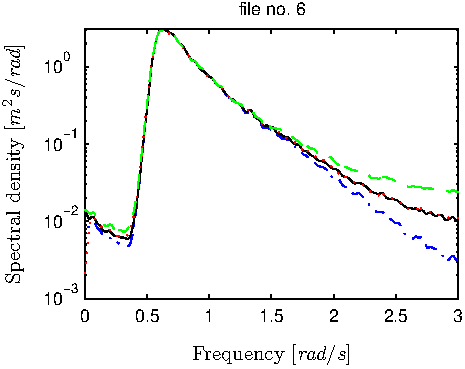
\includegraphics[width=3in]{spec6comparisonNew} %
%  \end{minipage} %
    \caption{Target spectrum, $S_{T}(\w)$, (solid) and its linear
  component, $S_{L}(\w)$ (dash-dot) compared with
$S_{T}^{NLS}$ (dash) and $S_{L}^{NLS}$ (dot), \ie{}
spectra of non-linearly simulated data using input
spectrum $S_{T}(\w)$ (method 1) and
$S_{L}(\w)$ (method 2), respectively.}
 \label{fig:spec6comparison} %
\end{figure}

Fig.\ref{fig:spec6comparison} demonstrates the differences in the
spectra obtained from data simulated using these methods. The solid
line is the target spectrum, $S_{T}(\w)$, and the dash-dotted line is
its linear component, $S_{L}(\w)$, obtained using
method 2.
The spectra $S_{T}^{NLS}$ (dashed) and
$S_{L}^{NLS}$ (dotted) are estimated from non-linearly simulated
data using the $S_{T}(\w)$ and $S_{L}(\w)$ spectra, respectively.
As expected $S_{T}^{NLS}$ is higher than
$S_{T}$, while  $S_{L}^{NLS}$ is indistinguishable from $S_{T}$.
It is also worth noting that the difference between the spectra is
small, but have some impact on the
higher order moments. For instance, the $\epsilon_{2}$ and  $\epsilon_{4}$ parameters
calculated from $S_{T}^{NLS}$ increase with $6.1\%$ and $2.5\%$,
respectively. The corresponding values calculated from $S_{L}^{NLS}$
increase with only  $0.5\%$ and $0.2\%$, respectively.

The small difference between  $S_{T}(\w)$ and $S_{L}(\w)$ also lends
some support to the view noted earlier, that
the difference frequency effect can not fully
explain the high values of the spectrum in the lower frequency part as
found by \cite{Wist2003Statistical}.

The effects these methods have are discussed further in
\cite{Brodtkorb2004Probability} and especially on  wave steepness
parameters. %wave-parameter characteristics.
The second order non-linear model explained here
is implemented in WAFO
 as \verb+spec2nlsdat.m+.
This is a very efficient implementation that calculate
 Eqs.~(\ref{eq:nonlinearcomponent}) to (\ref{eq:EsumAndEdiff}) in the
 bi-frequency domain using a one-dimensional \textit{FFT}.
This is similar to the \textit{WAVSIM} program of
\cite{NestegardAndStokka1995Third}, but is made even more efficient
 by summing over non-zero spectral values only and by eliminating the
 need for saving the computed results to the hard drive.
\textit{WAVSIM} use $40\, s$ to evaluate a transform with
$32000$ time steps/frequencies compared with $2\, s$ for
\verb+spec2nlsdat.m+ on a Pentium M
$1700$~\textit{MHz} with $1$~\textit{GB} of RAM.
Thus the use of second order random waves should now become common in ocean
engineering practice.

\verb+spec2nlsdat.m+ also allows finite water depth and any spectrum
as input, in contrast to
\textit{WAVSIM}, which only uses infinite water depth and the JONSWAP spectrum.

\section{Transformed linear Gaussian model}
\label{sec:transf-line-gauss}
An alternative and faster method than including the quadratic terms to
the linear model, is to use a transformation.
The non-Gaussian process, $\eta(x,t)$,
is then a function of a single Gaussian process, $\eta_{l}(x,t)$
\begin{equation} \label{eq:tran1}
  \eta(x,t)=G(\eta_{l}(x,t))
\end{equation}
where $G(\cdot)$ is a continuously differentiable function with positive
derivative.

There are several ways to proceed when selecting the
transformation. The simplest alternative is to estimate $G(\cdot)$
by some parametric or non-parametric means
(see \eg{} \cite{Winterstein1988Nonlinear,OchiAndAhn1994NonGaussian,RychlikEtal1997Modelling}).

The parametric formulas proposed by \cite{OchiAndAhn1994NonGaussian} as well as
\cite{Winterstein1988Nonlinear} use the moments of $\eta_{l}(x,t)$ to compute
$G(\cdot)$. Information about the moments can be obtained directly
from data or by using theoretical models.
\cite{MarthinsenAndWinterstein1992Skewness} derived an expression for the
skewness and kurtosis of narrow banded Stokes waves to the leading
order and used these to define the
transformation. \cite{WintersteinAndJha1995Random} fitted a
parametric model to skewness
and kurtosis of a second order model with a JONSWAP spectrum.

\cite{Machado2003Probability} studied the performance of 6
transformation methods including those mentioned above and concluded
that the Hermite method in general produces very good results.
%Thus, we only consider the  parametric Hermite model and use the
%estimated moments from data rather than those predicted by second order
%theory as suggested by \cite{JhaAndWinterstein2000Nonlinear}.

\subsection{Hermite model}
The Hermite transformation model proposed by
\cite{Winterstein1985Nonnormal}
%\cite{Winterstein1988Nonlinear}
approximates the true process by the following transformation of a
standard normal process $Y(t)$:
\begin{gather}
  G(y) = \mu + K \,\sigma \,[ y + c_{3}(y^2-1) + c_{4} \,(y^3-3\,y)] \\
%\intertext{where}
     K  = 1/\sqrt{1+2\,c_{3}^2+6\,c_{4}^2}
\end{gather}
where $\mu$ and $\sigma$ are the mean and standard deviation,
respectively,  of the true process. The unitless coefficients $c_{3}$ and
$c_{4}$ are chosen so that the transformed model
match the skewness, $\rho_{3}$, and excess,
$\rho_{4}$, of the true process.
%Earliest versions of this model \citep{Winterstein1985Nonnormal} assumed small
%non-linearity,
%for which
%\begin{align}
%c_{3} &\approx \rho_{3}/6 \\
%c_{4} &\approx (\rho_{4}-3)/24
%\end{align}
%a Hermite expansion of a Gaussian
%process $Y$ with zero mean and variance equal to one.
%The coefficients of resulting monotonic cubic polynomial is calibrated such
%that the first 4 moments of the transformed model $G(y)=g^-1(y)$
%match the moments of the true process.
%If the $\rho_{4}<3$ (hardening model)
%(shorter tails than a Gaussian distribution)
%\begin{gather}
%     g(x) =  xn - c3\,(xn^2-1) - c4\,(xn^3-3\,xn)
%\intertext{  where }
%    xn = (x-\mu)/\sigma
%    c3 = \rho_{3}/6
%    c4 = (\rho_{4}-3)/24
%\end{gather}
%  If $\rho_{4}>=3$ (softening model)
%(longer tails than a Gaussian distribution)
%\cite{Winterstein1988Nonlinear} improved the parameterizations.
\cite{WintersteinEtal1994Springing} improved the parameterizations by
minimizing lack-of-fit errors on $\rho_{3}$ and $\rho_{4}$, giving
\begin{align}
     c_{3}  &= \frac{\rho_{3}}{6} \,
\frac{1-0.015\,|\rho_{3}|+ 0.3\, \rho_{3}^2}{1+0.2\,\rho_{4}} \\
     c_{4}  &= 0.1\,\left( \left( 1+1.25\,\rho_{4} \right)^{1/3}-1 \right)\,c_{41}                 \\
     c_{41} &= \left(1-\frac{1.43\,\rho_{3}^2}{\rho_{4}} \right)^{1-0.1\,(\rho_{4}+3)^{0.8}}
\end{align}
These results apply for $0\le 3/2\,\rho_{3}^{2}<\rho_{4}<12$,
which include most cases
of practical interest.
%In section~\ref{sec:simulationStudy} we will
One may then estimate $c_{3}$ and $c_{4}$ using the sample
skewness, $\hat{\rho}_{3}$, but restrict $\rho_{4}$ so that
$\rho_{4} =
\min(\max(3\,\hat{\rho}_{3}^{2}/2,\hat{\rho}_{4}),\min(4\,(4\hat{\rho}_{3}/3)^{2},12))$.
$\hat{\rho}_{4}$ is the sample excess and
$(4\hat{\rho}_{3}/3)^{2}$ is the leading excess
contribution for narrow banded Stokes waves as found by
\cite{MarthinsenAndWinterstein1992Skewness}.


%%% Local Variables:
%%% mode: latex
%%% TeX-master: "wafomanual"
%%% End:
